% Options for packages loaded elsewhere
\PassOptionsToPackage{unicode}{hyperref}
\PassOptionsToPackage{hyphens}{url}
%
\documentclass[
]{book}
\usepackage{amsmath,amssymb}
\usepackage{iftex}
\ifPDFTeX
  \usepackage[T1]{fontenc}
  \usepackage[utf8]{inputenc}
  \usepackage{textcomp} % provide euro and other symbols
\else % if luatex or xetex
  \usepackage{unicode-math} % this also loads fontspec
  \defaultfontfeatures{Scale=MatchLowercase}
  \defaultfontfeatures[\rmfamily]{Ligatures=TeX,Scale=1}
\fi
\usepackage{lmodern}
\ifPDFTeX\else
  % xetex/luatex font selection
\fi
% Use upquote if available, for straight quotes in verbatim environments
\IfFileExists{upquote.sty}{\usepackage{upquote}}{}
\IfFileExists{microtype.sty}{% use microtype if available
  \usepackage[]{microtype}
  \UseMicrotypeSet[protrusion]{basicmath} % disable protrusion for tt fonts
}{}
\makeatletter
\@ifundefined{KOMAClassName}{% if non-KOMA class
  \IfFileExists{parskip.sty}{%
    \usepackage{parskip}
  }{% else
    \setlength{\parindent}{0pt}
    \setlength{\parskip}{6pt plus 2pt minus 1pt}}
}{% if KOMA class
  \KOMAoptions{parskip=half}}
\makeatother
\usepackage{xcolor}
\usepackage{color}
\usepackage{fancyvrb}
\newcommand{\VerbBar}{|}
\newcommand{\VERB}{\Verb[commandchars=\\\{\}]}
\DefineVerbatimEnvironment{Highlighting}{Verbatim}{commandchars=\\\{\}}
% Add ',fontsize=\small' for more characters per line
\usepackage{framed}
\definecolor{shadecolor}{RGB}{248,248,248}
\newenvironment{Shaded}{\begin{snugshade}}{\end{snugshade}}
\newcommand{\AlertTok}[1]{\textcolor[rgb]{0.94,0.16,0.16}{#1}}
\newcommand{\AnnotationTok}[1]{\textcolor[rgb]{0.56,0.35,0.01}{\textbf{\textit{#1}}}}
\newcommand{\AttributeTok}[1]{\textcolor[rgb]{0.13,0.29,0.53}{#1}}
\newcommand{\BaseNTok}[1]{\textcolor[rgb]{0.00,0.00,0.81}{#1}}
\newcommand{\BuiltInTok}[1]{#1}
\newcommand{\CharTok}[1]{\textcolor[rgb]{0.31,0.60,0.02}{#1}}
\newcommand{\CommentTok}[1]{\textcolor[rgb]{0.56,0.35,0.01}{\textit{#1}}}
\newcommand{\CommentVarTok}[1]{\textcolor[rgb]{0.56,0.35,0.01}{\textbf{\textit{#1}}}}
\newcommand{\ConstantTok}[1]{\textcolor[rgb]{0.56,0.35,0.01}{#1}}
\newcommand{\ControlFlowTok}[1]{\textcolor[rgb]{0.13,0.29,0.53}{\textbf{#1}}}
\newcommand{\DataTypeTok}[1]{\textcolor[rgb]{0.13,0.29,0.53}{#1}}
\newcommand{\DecValTok}[1]{\textcolor[rgb]{0.00,0.00,0.81}{#1}}
\newcommand{\DocumentationTok}[1]{\textcolor[rgb]{0.56,0.35,0.01}{\textbf{\textit{#1}}}}
\newcommand{\ErrorTok}[1]{\textcolor[rgb]{0.64,0.00,0.00}{\textbf{#1}}}
\newcommand{\ExtensionTok}[1]{#1}
\newcommand{\FloatTok}[1]{\textcolor[rgb]{0.00,0.00,0.81}{#1}}
\newcommand{\FunctionTok}[1]{\textcolor[rgb]{0.13,0.29,0.53}{\textbf{#1}}}
\newcommand{\ImportTok}[1]{#1}
\newcommand{\InformationTok}[1]{\textcolor[rgb]{0.56,0.35,0.01}{\textbf{\textit{#1}}}}
\newcommand{\KeywordTok}[1]{\textcolor[rgb]{0.13,0.29,0.53}{\textbf{#1}}}
\newcommand{\NormalTok}[1]{#1}
\newcommand{\OperatorTok}[1]{\textcolor[rgb]{0.81,0.36,0.00}{\textbf{#1}}}
\newcommand{\OtherTok}[1]{\textcolor[rgb]{0.56,0.35,0.01}{#1}}
\newcommand{\PreprocessorTok}[1]{\textcolor[rgb]{0.56,0.35,0.01}{\textit{#1}}}
\newcommand{\RegionMarkerTok}[1]{#1}
\newcommand{\SpecialCharTok}[1]{\textcolor[rgb]{0.81,0.36,0.00}{\textbf{#1}}}
\newcommand{\SpecialStringTok}[1]{\textcolor[rgb]{0.31,0.60,0.02}{#1}}
\newcommand{\StringTok}[1]{\textcolor[rgb]{0.31,0.60,0.02}{#1}}
\newcommand{\VariableTok}[1]{\textcolor[rgb]{0.00,0.00,0.00}{#1}}
\newcommand{\VerbatimStringTok}[1]{\textcolor[rgb]{0.31,0.60,0.02}{#1}}
\newcommand{\WarningTok}[1]{\textcolor[rgb]{0.56,0.35,0.01}{\textbf{\textit{#1}}}}
\usepackage{longtable,booktabs,array}
\usepackage{calc} % for calculating minipage widths
% Correct order of tables after \paragraph or \subparagraph
\usepackage{etoolbox}
\makeatletter
\patchcmd\longtable{\par}{\if@noskipsec\mbox{}\fi\par}{}{}
\makeatother
% Allow footnotes in longtable head/foot
\IfFileExists{footnotehyper.sty}{\usepackage{footnotehyper}}{\usepackage{footnote}}
\makesavenoteenv{longtable}
\usepackage{graphicx}
\makeatletter
\def\maxwidth{\ifdim\Gin@nat@width>\linewidth\linewidth\else\Gin@nat@width\fi}
\def\maxheight{\ifdim\Gin@nat@height>\textheight\textheight\else\Gin@nat@height\fi}
\makeatother
% Scale images if necessary, so that they will not overflow the page
% margins by default, and it is still possible to overwrite the defaults
% using explicit options in \includegraphics[width, height, ...]{}
\setkeys{Gin}{width=\maxwidth,height=\maxheight,keepaspectratio}
% Set default figure placement to htbp
\makeatletter
\def\fps@figure{htbp}
\makeatother
\setlength{\emergencystretch}{3em} % prevent overfull lines
\providecommand{\tightlist}{%
  \setlength{\itemsep}{0pt}\setlength{\parskip}{0pt}}
\setcounter{secnumdepth}{5}
\usepackage{booktabs}
\usepackage{amsthm}
\makeatletter
\def\thm@space@setup{%
  \thm@preskip=8pt plus 2pt minus 4pt
  \thm@postskip=\thm@preskip
}
\makeatother
\ifLuaTeX
  \usepackage{selnolig}  % disable illegal ligatures
\fi
\usepackage[]{natbib}
\bibliographystyle{apalike}
\IfFileExists{bookmark.sty}{\usepackage{bookmark}}{\usepackage{hyperref}}
\IfFileExists{xurl.sty}{\usepackage{xurl}}{} % add URL line breaks if available
\urlstyle{same}
\hypersetup{
  pdftitle={A Minimal Book Example},
  pdfauthor={Yihui Xie},
  hidelinks,
  pdfcreator={LaTeX via pandoc}}

\title{A Minimal Book Example}
\author{Yihui Xie}
\date{2024-02-08}

\begin{document}
\maketitle

{
\setcounter{tocdepth}{1}
\tableofcontents
}
\hypertarget{prerequisites}{%
\chapter{Prerequisites}\label{prerequisites}}

This is a \emph{sample} book written in \textbf{Markdown}. You can use anything that Pandoc's Markdown supports, e.g., a math equation \(a^2 + b^2 = c^2\).

The \textbf{bookdown} package can be installed from CRAN or Github:

\begin{Shaded}
\begin{Highlighting}[]
\FunctionTok{install.packages}\NormalTok{(}\StringTok{"bookdown"}\NormalTok{)}
\CommentTok{\# or the development version}
\CommentTok{\# devtools::install\_github("rstudio/bookdown")}
\end{Highlighting}
\end{Shaded}

Remember each Rmd file contains one and only one chapter, and a chapter is defined by the first-level heading \texttt{\#}.

To compile this example to PDF, you need XeLaTeX. You are recommended to install TinyTeX (which includes XeLaTeX): \url{https://yihui.name/tinytex/}.

\hypertarget{intro}{%
\chapter{Introduction}\label{intro}}

You can label chapter and section titles using \texttt{\{\#label\}} after them, e.g., we can reference Chapter \ref{intro}. If you do not manually label them, there will be automatic labels anyway, e.g., Chapter \ref{methods}.

Figures and tables with captions will be placed in \texttt{figure} and \texttt{table} environments, respectively.

\begin{Shaded}
\begin{Highlighting}[]
\FunctionTok{par}\NormalTok{(}\AttributeTok{mar =} \FunctionTok{c}\NormalTok{(}\DecValTok{4}\NormalTok{, }\DecValTok{4}\NormalTok{, .}\DecValTok{1}\NormalTok{, .}\DecValTok{1}\NormalTok{))}
\FunctionTok{plot}\NormalTok{(pressure, }\AttributeTok{type =} \StringTok{\textquotesingle{}b\textquotesingle{}}\NormalTok{, }\AttributeTok{pch =} \DecValTok{19}\NormalTok{)}
\end{Highlighting}
\end{Shaded}

\begin{figure}

{\centering 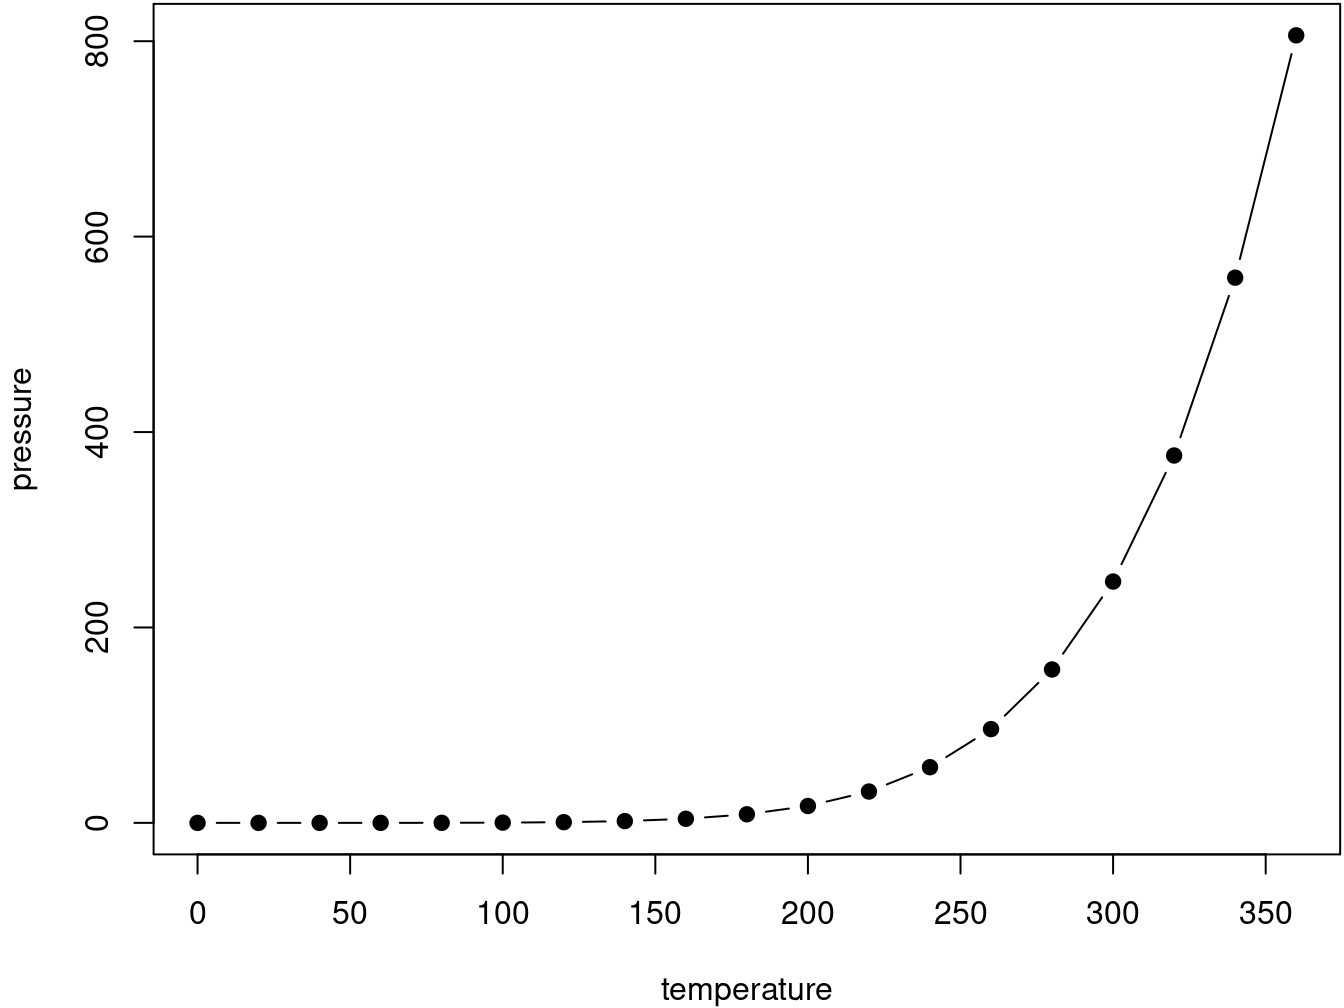
\includegraphics[width=0.8\linewidth]{rechaRge-book_files/figure-latex/nice-fig-1} 

}

\caption{Here is a nice figure!}\label{fig:nice-fig}
\end{figure}

Reference a figure by its code chunk label with the \texttt{fig:} prefix, e.g., see Figure \ref{fig:nice-fig}. Similarly, you can reference tables generated from \texttt{knitr::kable()}, e.g., see Table \ref{tab:nice-tab}.

\begin{Shaded}
\begin{Highlighting}[]
\NormalTok{knitr}\SpecialCharTok{::}\FunctionTok{kable}\NormalTok{(}
  \FunctionTok{head}\NormalTok{(iris, }\DecValTok{20}\NormalTok{), }\AttributeTok{caption =} \StringTok{\textquotesingle{}Here is a nice table!\textquotesingle{}}\NormalTok{,}
  \AttributeTok{booktabs =} \ConstantTok{TRUE}
\NormalTok{)}
\end{Highlighting}
\end{Shaded}

\begin{table}

\caption{\label{tab:nice-tab}Here is a nice table!}
\centering
\begin{tabular}[t]{rrrrl}
\toprule
Sepal.Length & Sepal.Width & Petal.Length & Petal.Width & Species\\
\midrule
5.1 & 3.5 & 1.4 & 0.2 & setosa\\
4.9 & 3.0 & 1.4 & 0.2 & setosa\\
4.7 & 3.2 & 1.3 & 0.2 & setosa\\
4.6 & 3.1 & 1.5 & 0.2 & setosa\\
5.0 & 3.6 & 1.4 & 0.2 & setosa\\
\addlinespace
5.4 & 3.9 & 1.7 & 0.4 & setosa\\
4.6 & 3.4 & 1.4 & 0.3 & setosa\\
5.0 & 3.4 & 1.5 & 0.2 & setosa\\
4.4 & 2.9 & 1.4 & 0.2 & setosa\\
4.9 & 3.1 & 1.5 & 0.1 & setosa\\
\addlinespace
5.4 & 3.7 & 1.5 & 0.2 & setosa\\
4.8 & 3.4 & 1.6 & 0.2 & setosa\\
4.8 & 3.0 & 1.4 & 0.1 & setosa\\
4.3 & 3.0 & 1.1 & 0.1 & setosa\\
5.8 & 4.0 & 1.2 & 0.2 & setosa\\
\addlinespace
5.7 & 4.4 & 1.5 & 0.4 & setosa\\
5.4 & 3.9 & 1.3 & 0.4 & setosa\\
5.1 & 3.5 & 1.4 & 0.3 & setosa\\
5.7 & 3.8 & 1.7 & 0.3 & setosa\\
5.1 & 3.8 & 1.5 & 0.3 & setosa\\
\bottomrule
\end{tabular}
\end{table}

You can write citations, too. For example, we are using the \textbf{bookdown} package \citep{R-bookdown} in this sample book, which was built on top of R Markdown and \textbf{knitr} \citep{xie2015}.

\hypertarget{literature}{%
\chapter{Literature}\label{literature}}

Here is a review of existing methods.

\hypertarget{methods}{%
\chapter{Methods}\label{methods}}

We describe our methods in this chapter.

Math can be added in body using usual syntax like this

\hypertarget{math-example}{%
\section{math example}\label{math-example}}

\(p\) is unknown but expected to be around 1/3. Standard error will be approximated

\[
SE = \sqrt(\frac{p(1-p)}{n}) \approx \sqrt{\frac{1/3 (1 - 1/3)} {300}} = 0.027
\]

You can also use math in footnotes like this\footnote{where we mention \(p = \frac{a}{b}\)}.

We will approximate standard error to 0.027\footnote{\(p\) is unknown but expected to be around 1/3. Standard error will be approximated

  \[
  SE = \sqrt(\frac{p(1-p)}{n}) \approx \sqrt{\frac{1/3 (1 - 1/3)} {300}} = 0.027
  \]}

\hypertarget{example}{%
\chapter{Example}\label{example}}

Load the \emph{rechaRge} library.

\begin{Shaded}
\begin{Highlighting}[]
\FunctionTok{library}\NormalTok{(rechaRge)}
\end{Highlighting}
\end{Shaded}

\hypertarget{hydrobudget-model}{%
\section{HydroBudget model}\label{hydrobudget-model}}

\hypertarget{input-data-and-parameters}{%
\subsection{Input data and parameters}\label{input-data-and-parameters}}

Load the input data for the simulation.

\begin{Shaded}
\begin{Highlighting}[]
\NormalTok{base\_url }\OtherTok{\textless{}{-}} \StringTok{"https://github.com/gwrecharge/rechaRge{-}book/raw/main/examples/input/"}
\NormalTok{input\_rcn }\OtherTok{\textless{}{-}} \FunctionTok{paste0}\NormalTok{(base\_url, }\StringTok{"rcn.csv.gz"}\NormalTok{) }\CommentTok{\# RCN values per RCN cell ID}
\NormalTok{input\_climate }\OtherTok{\textless{}{-}} \FunctionTok{paste0}\NormalTok{(base\_url, }\StringTok{"climate.csv.gz"}\NormalTok{) }\CommentTok{\# precipitation total in mm/d per climate cell ID}
\NormalTok{input\_rcn\_climate }\OtherTok{\textless{}{-}} \FunctionTok{paste0}\NormalTok{(base\_url, }\StringTok{"rcn\_climate.csv.gz"}\NormalTok{) }\CommentTok{\# relation between climate and RCN cell IDs}
\NormalTok{input\_rcn\_gauging }\OtherTok{\textless{}{-}} \FunctionTok{paste0}\NormalTok{(base\_url, }\StringTok{"rcn\_gauging.csv.gz"}\NormalTok{) }\CommentTok{\# relation between gaugins station and RCN cell IDs}
\NormalTok{input\_observed\_flow }\OtherTok{\textless{}{-}} \FunctionTok{paste0}\NormalTok{(base\_url, }\StringTok{"observed\_flow.csv.gz"}\NormalTok{) }\CommentTok{\# flow rates in mm/d}
\NormalTok{input\_alpha\_lyne\_hollick }\OtherTok{\textless{}{-}} \FunctionTok{paste0}\NormalTok{(base\_url, }\StringTok{"alpha\_lyne\_hollick.csv.gz"}\NormalTok{)}
\end{Highlighting}
\end{Shaded}

Set the \textbf{HydroBudget} model with the parameters values:

\begin{Shaded}
\begin{Highlighting}[]
\NormalTok{HB }\OtherTok{\textless{}{-}}\NormalTok{ rechaRge}\SpecialCharTok{::}\FunctionTok{new\_hydrobugdet}\NormalTok{(}
  \AttributeTok{T\_m =} \FloatTok{2.1}\NormalTok{, }\CommentTok{\# melting temperature (°C)}
  \AttributeTok{C\_m =} \FloatTok{6.2}\NormalTok{, }\CommentTok{\# melting coefficient (mm/°C/d)}
  \AttributeTok{TT\_F =} \SpecialCharTok{{-}}\FloatTok{17.6}\NormalTok{, }\CommentTok{\# Threshold temperature for soil frost (°C)}
  \AttributeTok{F\_T =} \FloatTok{16.4}\NormalTok{, }\CommentTok{\# Freezing time (d)}
  \AttributeTok{t\_API =} \FloatTok{3.9}\NormalTok{, }\CommentTok{\# Antecedent precipitation index time (d)}
  \AttributeTok{f\_runoff =} \FloatTok{0.63}\NormalTok{, }\CommentTok{\# Runoff factor ({-})}
  \AttributeTok{sw\_m =} \DecValTok{431}\NormalTok{, }\CommentTok{\# Maximum soil water content (mm)}
  \AttributeTok{f\_inf =} \FloatTok{0.07} \CommentTok{\# infiltration factor ({-})}
\NormalTok{)}
\end{Highlighting}
\end{Shaded}

Set the column names mappings matching the input datasets:

\begin{Shaded}
\begin{Highlighting}[]
\NormalTok{HB}\SpecialCharTok{$}\NormalTok{rcn\_columns }\OtherTok{\textless{}{-}} \FunctionTok{list}\NormalTok{(}
  \AttributeTok{rcn\_id =} \StringTok{"cell\_ID"}\NormalTok{,}
  \AttributeTok{RCNII =} \StringTok{"RCNII"}\NormalTok{,}
  \AttributeTok{lon =} \StringTok{"X\_L93"}\NormalTok{,}
  \AttributeTok{lat =} \StringTok{"Y\_L93"}
\NormalTok{)}
\NormalTok{HB}\SpecialCharTok{$}\NormalTok{climate\_columns}\SpecialCharTok{$}\NormalTok{climate\_id }\OtherTok{\textless{}{-}} \StringTok{"climate\_cell"}
\NormalTok{HB}\SpecialCharTok{$}\NormalTok{rcn\_climate\_columns }\OtherTok{\textless{}{-}} \FunctionTok{list}\NormalTok{(}
  \AttributeTok{climate\_id =} \StringTok{"climate\_cell"}\NormalTok{,}
  \AttributeTok{rcn\_id =} \StringTok{"cell\_ID"}
\NormalTok{)}
\NormalTok{HB}\SpecialCharTok{$}\NormalTok{rcn\_gauging\_columns }\OtherTok{\textless{}{-}} \FunctionTok{list}\NormalTok{(}
  \AttributeTok{rcn\_id =} \StringTok{"cell\_ID"}\NormalTok{,}
  \AttributeTok{station\_id =} \StringTok{"gauging\_stat"}
\NormalTok{)}
\NormalTok{HB}\SpecialCharTok{$}\NormalTok{alpha\_lyne\_hollick\_columns}\SpecialCharTok{$}\NormalTok{station\_id }\OtherTok{\textless{}{-}} \StringTok{"station"}
\end{Highlighting}
\end{Shaded}

Set the simulation period:

\begin{Shaded}
\begin{Highlighting}[]
\NormalTok{simul\_period }\OtherTok{\textless{}{-}} \FunctionTok{c}\NormalTok{(}\DecValTok{2010}\NormalTok{, }\DecValTok{2017}\NormalTok{)}
\end{Highlighting}
\end{Shaded}

\hypertarget{simulation}{%
\subsection{Simulation}\label{simulation}}

Compute the water budget using the HydroBudget model:

\begin{Shaded}
\begin{Highlighting}[]
\NormalTok{water\_budget }\OtherTok{\textless{}{-}}\NormalTok{ rechaRge}\SpecialCharTok{::}\FunctionTok{compute\_recharge}\NormalTok{(}
\NormalTok{  HB,}
  \AttributeTok{rcn =}\NormalTok{ input\_rcn,}
  \AttributeTok{climate =}\NormalTok{ input\_climate,}
  \AttributeTok{rcn\_climate =}\NormalTok{ input\_rcn\_climate,}
  \AttributeTok{period =}\NormalTok{ simul\_period}
\NormalTok{)}
\end{Highlighting}
\end{Shaded}

The water budget data set is per year-month in each RCN cell:

\begin{itemize}
\tightlist
\item
  \texttt{vi}, the vertical inflow
\item
  \texttt{t\_mean}, the mean temperature
\item
  \texttt{runoff}, the runoff
\item
  \texttt{pet}, the potential evapotranspiration
\item
  \texttt{aet}, the actual evapotranspiration
\item
  \texttt{gwr}, the ground water recharge
\item
  \texttt{runoff\_2}, the excess runoff
\end{itemize}

The head of this data set is:

\begin{tabular}{r|r|r|r|r|r|r|r|r|r|r}
\hline
year & month & vi & t\_mean & runoff & pet & aet & gwr & runoff\_2 & delta\_reservoir & rcn\_id\\
\hline
2010 & 1 & 28.2 & -7.3 & 21.5 & 1.6 & 1.6 & 10.2 & 0 & -5.1 & 62097\\
\hline
2010 & 2 & 27.9 & -5.7 & 7.9 & 4.6 & 4.6 & 8.8 & 0 & 6.6 & 62097\\
\hline
2010 & 3 & 83.0 & 1.0 & 30.8 & 19.5 & 19.5 & 16.1 & 0 & 16.6 & 62097\\
\hline
2010 & 4 & 68.2 & 7.7 & 24.9 & 51.5 & 51.5 & 15.1 & 0 & -23.3 & 62097\\
\hline
2010 & 5 & 46.9 & 13.8 & 3.8 & 94.7 & 73.8 & 4.4 & 0 & -35.2 & 62097\\
\hline
2010 & 6 & 107.9 & 17.0 & 33.3 & 114.7 & 81.1 & 0.2 & 0 & -6.7 & 62097\\
\hline
\end{tabular}

\hypertarget{quality-assessment}{%
\subsection{Quality assessment}\label{quality-assessment}}

Process the river flow observations and assess simulation quality:

\begin{Shaded}
\begin{Highlighting}[]
\NormalTok{result }\OtherTok{\textless{}{-}}\NormalTok{ rechaRge}\SpecialCharTok{::}\FunctionTok{compute\_simulation\_quality\_assessment}\NormalTok{(}
\NormalTok{  HB,}
  \AttributeTok{water\_budget =}\NormalTok{ water\_budget,}
  \AttributeTok{rcn\_gauging =}\NormalTok{ input\_rcn\_gauging,}
  \AttributeTok{observed\_flow =}\NormalTok{ input\_observed\_flow,}
  \AttributeTok{alpha\_lyne\_hollick =}\NormalTok{ input\_alpha\_lyne\_hollick,}
  \AttributeTok{period =}\NormalTok{ simul\_period}
\NormalTok{)}
\end{Highlighting}
\end{Shaded}

\hypertarget{results-handling}{%
\subsection{Results handling}\label{results-handling}}

Save the simulation results:

\begin{Shaded}
\begin{Highlighting}[]
\NormalTok{sim\_dir }\OtherTok{\textless{}{-}} \FunctionTok{file.path}\NormalTok{(}\FunctionTok{tempdir}\NormalTok{(), }\FunctionTok{paste0}\NormalTok{(}\StringTok{"simulation\_HydroBudget\_"}\NormalTok{, }\FunctionTok{format}\NormalTok{(}\FunctionTok{Sys.time}\NormalTok{(), }\StringTok{"\%Y\%m\%dT\%H\_\%M"}\NormalTok{)))}

\CommentTok{\# Write output files}
\CommentTok{\# CSV}
\NormalTok{rechaRge}\SpecialCharTok{::}\FunctionTok{write\_recharge\_results}\NormalTok{(HB, water\_budget, }\AttributeTok{output\_dir =}\NormalTok{ sim\_dir)}
\CommentTok{\# NetCDF}
\NormalTok{rechaRge}\SpecialCharTok{::}\FunctionTok{write\_recharge\_results}\NormalTok{(HB, water\_budget, }\AttributeTok{output\_dir =}\NormalTok{ sim\_dir, }\AttributeTok{format =} \StringTok{"nc"}\NormalTok{, }\AttributeTok{input\_rcn =}\NormalTok{ input\_rcn, }\AttributeTok{names =} \FunctionTok{list}\NormalTok{(}
  \StringTok{"lon"} \OtherTok{=} \FunctionTok{list}\NormalTok{(}
    \AttributeTok{longname =} \StringTok{"Qc lambert NAD83 epsg32198 Est"}\NormalTok{,}
    \AttributeTok{unit =} \StringTok{"m"}
\NormalTok{  ),}
  \StringTok{"lat"} \OtherTok{=} \FunctionTok{list}\NormalTok{(}
    \AttributeTok{longname =} \StringTok{"Qc lambert NAD83 epsg32198 North"}\NormalTok{,}
    \AttributeTok{unit =} \StringTok{"m"}
\NormalTok{  )}
\NormalTok{))}
\CommentTok{\# Rasters}
\NormalTok{rechaRge}\SpecialCharTok{::}\FunctionTok{write\_recharge\_rasters}\NormalTok{(}
\NormalTok{  HB,}
  \AttributeTok{water\_budget =}\NormalTok{ water\_budget,}
  \AttributeTok{input\_rcn =}\NormalTok{ input\_rcn,}
  \AttributeTok{crs =} \StringTok{"+proj=lcc +lat\_1=60 +lat\_2=46 +lat\_0=44 +lon\_0={-}68.5 +x\_0=0 +y\_0=0 +ellps=GRS80 +datum=NAD83 +units=m +no\_defs"}\NormalTok{,}
  \AttributeTok{output\_dir =}\NormalTok{ sim\_dir}
\NormalTok{)}


\CommentTok{\# List simulation output files}
\FunctionTok{list.files}\NormalTok{(sim\_dir)}
\end{Highlighting}
\end{Shaded}

\begin{verbatim}
## [1] "bilan_spat_month.csv"         "bilan_unspat_month.csv"      
## [3] "interannual_aet_NAD83.tif"    "interannual_gwr_NAD83.tif"   
## [5] "interannual_runoff_NAD83.tif" "water_budget.nc"
\end{verbatim}

\hypertarget{data-visualization}{%
\subsection{Data visualization}\label{data-visualization}}

Visualize the saved NetCDF file:

\begin{Shaded}
\begin{Highlighting}[]
\FunctionTok{library}\NormalTok{(ncdf4)}
\FunctionTok{library}\NormalTok{(lattice)}
\FunctionTok{library}\NormalTok{(viridisLite)}

\CommentTok{\# Extract GWR data}
\NormalTok{nc }\OtherTok{\textless{}{-}} \FunctionTok{nc\_open}\NormalTok{(}\FunctionTok{file.path}\NormalTok{(sim\_dir, }\StringTok{"water\_budget.nc"}\NormalTok{))}
\NormalTok{gwr }\OtherTok{\textless{}{-}} \FunctionTok{ncvar\_get}\NormalTok{(nc, }\StringTok{"gwr"}\NormalTok{)}
\NormalTok{lon }\OtherTok{\textless{}{-}} \FunctionTok{ncvar\_get}\NormalTok{(nc, }\StringTok{"lon"}\NormalTok{)}
\NormalTok{lat }\OtherTok{\textless{}{-}} \FunctionTok{ncvar\_get}\NormalTok{(nc, }\StringTok{"lat"}\NormalTok{)}
\NormalTok{time }\OtherTok{\textless{}{-}} \FunctionTok{ncvar\_get}\NormalTok{(nc, }\StringTok{"time"}\NormalTok{)}
\FunctionTok{nc\_close}\NormalTok{(nc)}

\CommentTok{\# Render the 18th month}
\NormalTok{gwr1 }\OtherTok{\textless{}{-}}\NormalTok{ gwr[,,}\DecValTok{18}\NormalTok{]}
\NormalTok{grid }\OtherTok{\textless{}{-}} \FunctionTok{expand.grid}\NormalTok{(}\AttributeTok{lon=}\NormalTok{lon, }\AttributeTok{lat=}\NormalTok{lat)}
\FunctionTok{levelplot}\NormalTok{(gwr1 }\SpecialCharTok{\textasciitilde{}}\NormalTok{ lon }\SpecialCharTok{*}\NormalTok{ lat, }\AttributeTok{data=}\NormalTok{grid, }\AttributeTok{pretty=}\NormalTok{T, }\AttributeTok{col.regions=}\FunctionTok{magma}\NormalTok{(}\DecValTok{100}\NormalTok{))}
\end{Highlighting}
\end{Shaded}

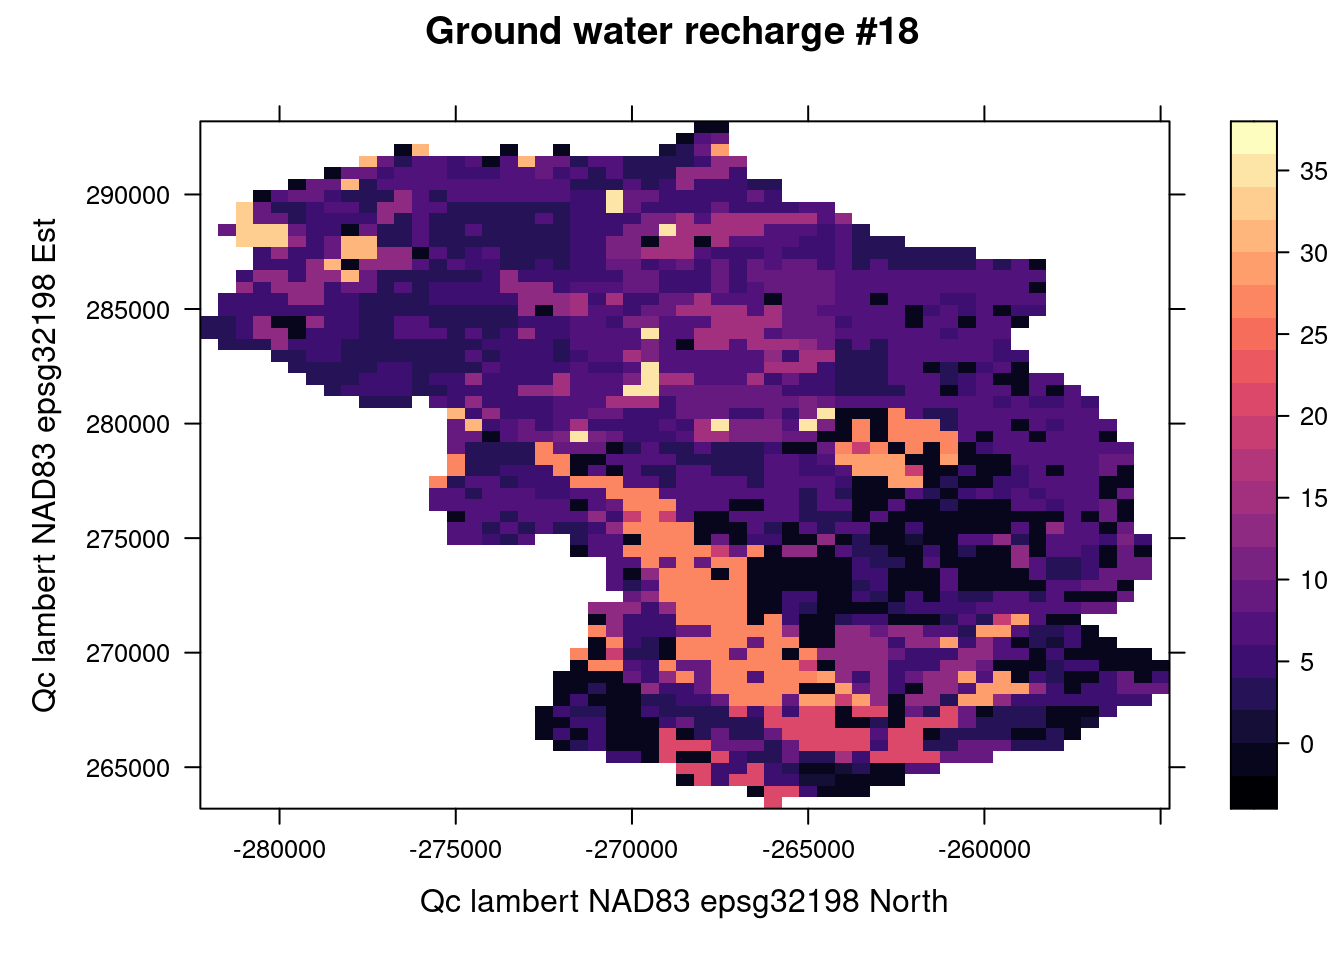
\includegraphics{rechaRge-book_files/figure-latex/unnamed-chunk-12-1.pdf}

Visualize the saved raster files:

\begin{Shaded}
\begin{Highlighting}[]
\FunctionTok{library}\NormalTok{(tidyterra)}
\FunctionTok{library}\NormalTok{(terra)}
\FunctionTok{library}\NormalTok{(ggplot2)}
\FunctionTok{library}\NormalTok{(cowplot)}
\NormalTok{subtitle }\OtherTok{\textless{}{-}} \FunctionTok{ifelse}\NormalTok{(simul\_period[}\DecValTok{1}\NormalTok{] }\SpecialCharTok{==}\NormalTok{ simul\_period[}\DecValTok{2}\NormalTok{],}
  \FunctionTok{paste0}\NormalTok{(}\StringTok{"In "}\NormalTok{, simul\_period[}\DecValTok{1}\NormalTok{]),}
  \FunctionTok{paste0}\NormalTok{(}\StringTok{"From "}\NormalTok{, simul\_period[}\DecValTok{1}\NormalTok{], }\StringTok{" to "}\NormalTok{, simul\_period[}\DecValTok{2}\NormalTok{])}
\NormalTok{)}
\NormalTok{runoff }\OtherTok{\textless{}{-}}\NormalTok{ terra}\SpecialCharTok{::}\FunctionTok{rast}\NormalTok{(}\FunctionTok{file.path}\NormalTok{(sim\_dir, }\StringTok{"interannual\_runoff\_NAD83.tif"}\NormalTok{))}
\NormalTok{runoffplot }\OtherTok{\textless{}{-}} \FunctionTok{ggplot}\NormalTok{() }\SpecialCharTok{+}
  \FunctionTok{geom\_spatraster}\NormalTok{(}\AttributeTok{data =}\NormalTok{ runoff) }\SpecialCharTok{+}
  \FunctionTok{scale\_fill\_viridis\_c}\NormalTok{(}\AttributeTok{option =} \StringTok{"inferno"}\NormalTok{) }\SpecialCharTok{+}
  \FunctionTok{labs}\NormalTok{(}
    \AttributeTok{fill =} \StringTok{""}\NormalTok{,}
    \AttributeTok{title =} \StringTok{"Runoff"}\NormalTok{,}
    \AttributeTok{subtitle =}\NormalTok{ subtitle}
\NormalTok{  )}
\NormalTok{aet }\OtherTok{\textless{}{-}}\NormalTok{ terra}\SpecialCharTok{::}\FunctionTok{rast}\NormalTok{(}\FunctionTok{file.path}\NormalTok{(sim\_dir, }\StringTok{"interannual\_aet\_NAD83.tif"}\NormalTok{))}
\NormalTok{aetplot }\OtherTok{\textless{}{-}} \FunctionTok{ggplot}\NormalTok{() }\SpecialCharTok{+}
  \FunctionTok{geom\_spatraster}\NormalTok{(}\AttributeTok{data =}\NormalTok{ aet) }\SpecialCharTok{+}
  \FunctionTok{scale\_fill\_viridis\_c}\NormalTok{(}\AttributeTok{option =} \StringTok{"inferno"}\NormalTok{) }\SpecialCharTok{+}
  \FunctionTok{labs}\NormalTok{(}
    \AttributeTok{fill =} \StringTok{""}\NormalTok{,}
    \AttributeTok{title =} \StringTok{"Actual Evapotranspiration"}\NormalTok{,}
    \AttributeTok{subtitle =}\NormalTok{ subtitle}
\NormalTok{  )}
\NormalTok{gwr }\OtherTok{\textless{}{-}}\NormalTok{ terra}\SpecialCharTok{::}\FunctionTok{rast}\NormalTok{(}\FunctionTok{file.path}\NormalTok{(sim\_dir, }\StringTok{"interannual\_gwr\_NAD83.tif"}\NormalTok{))}
\NormalTok{gwrplot }\OtherTok{\textless{}{-}} \FunctionTok{ggplot}\NormalTok{() }\SpecialCharTok{+}
  \FunctionTok{geom\_spatraster}\NormalTok{(}\AttributeTok{data =}\NormalTok{ gwr) }\SpecialCharTok{+}
  \FunctionTok{scale\_fill\_viridis\_c}\NormalTok{(}\AttributeTok{option =} \StringTok{"inferno"}\NormalTok{) }\SpecialCharTok{+}
  \FunctionTok{labs}\NormalTok{(}
    \AttributeTok{fill =} \StringTok{""}\NormalTok{,}
    \AttributeTok{title =} \StringTok{"Ground Water Recharge"}\NormalTok{,}
    \AttributeTok{subtitle =}\NormalTok{ subtitle}
\NormalTok{  )}
\NormalTok{cowplot}\SpecialCharTok{::}\FunctionTok{plot\_grid}\NormalTok{(runoffplot, aetplot, gwrplot)}
\end{Highlighting}
\end{Shaded}

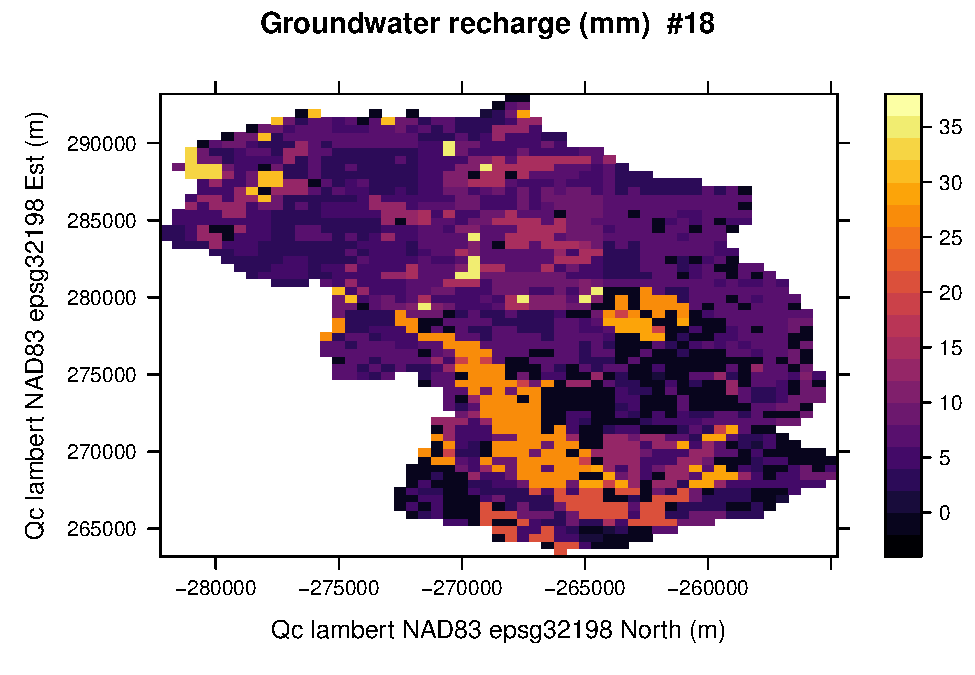
\includegraphics{rechaRge-book_files/figure-latex/unnamed-chunk-13-1.pdf}

\hypertarget{final-words}{%
\chapter{Final Words}\label{final-words}}

We have finished a nice book.

  \bibliography{book.bib,packages.bib}

\end{document}
